\section{Thermodynamique : calorimétrie et machines thermiques}

%UAA8-Chap 1-2-3-4, pages 162 à 185)

\subsection{Définition}~: La thermodynamique est la partie de la
physique qui étudie les transformations d'énergie impliquant l'énergie
thermique. En particulier, elle étudie comment convertir cette énergie
thermique en énergie mécanique~(moteur à combustion, machine à vapeur,
turbine, \ldots)

\subsection{Conservation de l'énergie et premier principe de la thermodynamique. }

\subsubsection{Mise en situation}}

\begin{itemize}
\item  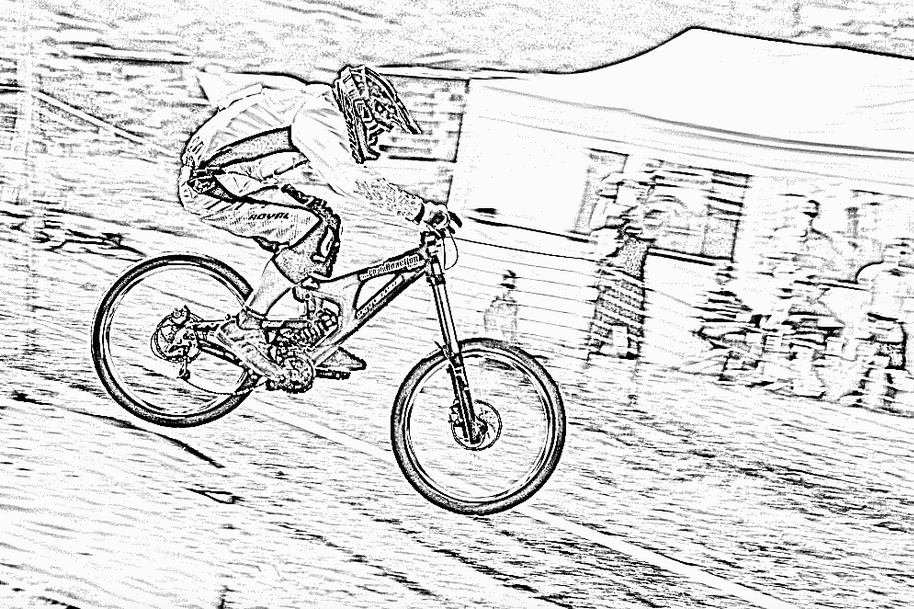
\includegraphics[width=2.829cm,height=2cm]{Pictures/1000000100000392000002617E5250701D3115A8.png}Frottez
  vous les mains~: vous transformez de l'énergie mécanique en énergie
  thermique.
\item  Freinez en descendant une pente à vélo~: les freins s'échauffent.
\item  Un engin spatial (la navette) effectue son retour dans l'atmosphère,
  il y a échauffement. L'engin doit être protégé pour éviter sa  destruction.
\end{itemize}

Nous voyons par ces exemples que de l'énergie mécanique (due au
mouvement) se transforme en énergie thermique.

\begin{figure}
\centering
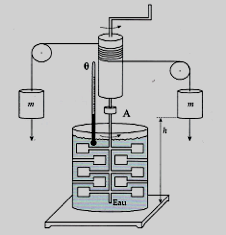
\includegraphics[width=5.544cm,height=5.777cm]{Pictures/10000001000000E2000000EB4F714951B1E3FFA5.png}
\caption{}
\end{figure}

%\subsection{Rappels de calorimétrie}
% (pages 162 à 167)

\subsubsection{Expérience de Joule}

En 1850, James Prescott Joule réalise une expérience mettant en évidence
de façon quantitative cet échange d'énergie mécanique en énergie
thermique.

Un récipient, isolé et rempli d'eau, contient des roues à palettes.
Comme le montre le schéma, les deux roues sont mises en rotation par la
chute de deux masses égales (il y a donc diminution de l'énergie
potentielle des deux masses). Joule observe une élévation de température
de l'eau (il y a donc augmentation de l'énergie thermique) et observe
expérimentalement ~que~:

\textsubscript{}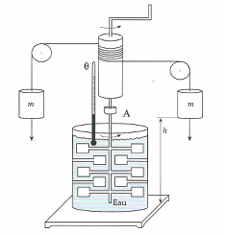
\includegraphics[width=1.835cm,height=0.989cm]{Pictures/10000001000000E2000000EB005D4F6E603818B5.png}
où cette constante notée c sera appelée la \textbf{chaleur massique}
(ici de l'eau).

\textbf{L'énergie mécanique perdue par le système~(E) est transformée
en énergie thermique qui se mesure par une élévation de température
(). }

Ce rapport c dépend de~:
\begin{itemize}
\item  la \emph{\textbf{quantité du liquide}} (ici de l'eau) dans le
  récipient.
\item  c dépend de la \emph{\textbf{nature du liquide}} (ici de l'eau, mais
  cela peut être de huile, de l'essence, \ldots{} )
\end{itemize}

E est la variation d'énergie mécanique qui est égale à la variation
d'énergie thermique. Nous noterons cette variation d'énergie thermique~:

Q

\subsubsection{Equation de la calorimétrie~(rappel)}

\begin{figure}
\centering
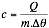
\includegraphics[width=1.742cm,height=0.989cm]{Pictures/10000001000000310000001C55B97172EC4D3DC9.png}
\caption{}
\end{figure}

\begin{itemize}
\item  Pour l'eau, si vous prenez 1 litre d'eau et que vous voulez augmenter
  sa température de 1°C, il faudra lui fournir une énergie thermique de
  4 186 J.
\item  Si vous comparez les chaleurs massiques de l'eau et de l'huile, vous
  voyez que l'huile «~chauffe plus facilement~» que l'eau. Il faudra
  fournir moins d'énergie thermique à 1 litre d'huile pour élever sa
  température de 1°C qu'à 1 litre d'eau pour élever sa température de
  1°C puisque la chaleur massique de l'huile est inférieure à celle de
  l'eau.
\item   Page 163 du livre , vous trouverez les chaleurs massiques de
  différentes substances.
  TODO TABLEAU A AJOUTER ICI 
\end{itemize}

\subsection{Premier principe de la thermodynamique~: principe de  conservation d'énergie. }

Définition~: Un \textbf{système isolé }est un système qui n'échange ni
matière, ni chaleur, ni travail avec l'extérieur.

En conséquence, si une partie du système isolé perd de l'énergie, une
autre partie du système en gagne une quantité identique.

\emph{Illustrations~: }
\begin{itemize}
\item  Lorsqu'une voiture freine, elle perd de l'énergie cinétique. Il doit y
  avoir une augmentation d'énergie dans le système. C'est de l'énergie
  thermique par échauffement des freins.
\item  Dans l'expérience de Joule, les masses perdent de l'énergie
  potentielle gravifique. Il doit y avoir une augmentation d'énergie
  dans le système. C'est de l'énergie thermique traduite par
  l'augmentation de température de l'eau.
\end{itemize}

\subsection{EXERCICE RESOLU A REALISER~: page 164-165 du livre.}

\begin{enumerate}
\item
  \emph{Rendement d'une transformation énergétique }
\end{enumerate}

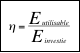
\includegraphics[width=3.108cm,height=2.073cm]{Pictures/10000001000000500000003510F712318EAE4AA8.png}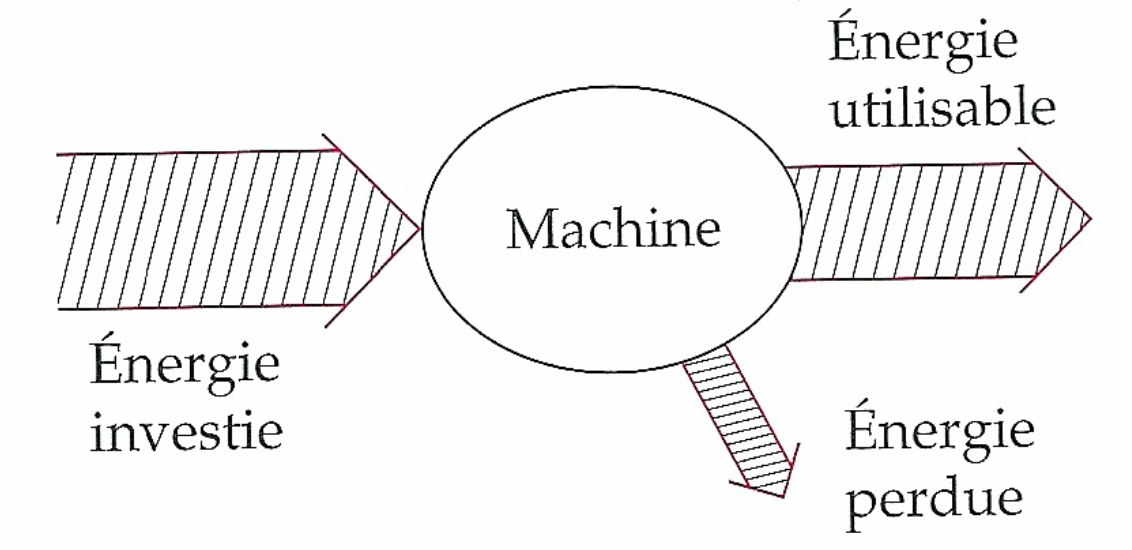
\includegraphics[width=5.95cm,height=2.896cm]{Pictures/100000010000046C00000226BB542474620E0092.png}

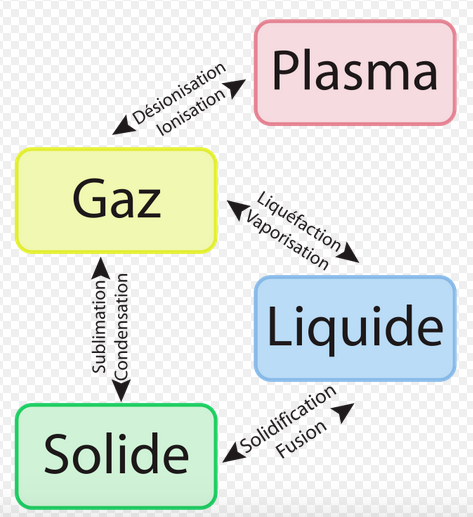
\includegraphics[width=5.184cm,height=4.166cm]{Pictures/10000001000001D9000002050D0008DD07AA637E.png}\emph{\textbf{A3-Echange
d'énergie lors d'un changement d'état. }}

En
\href{https://fr.wikipedia.org/wiki/Thermodynamique}{\emph{\emph{thermodynamique}}},
un \textbf{changement d'état} est le passage d'un
\href{https://fr.wikipedia.org/wiki/\%C3\%89tat_de_la_mati\%C3\%A8re}{\emph{\emph{état}}}
de la
\href{https://fr.wikipedia.org/wiki/Mati\%C3\%A8re}{\emph{\emph{matière}}}
à un autre état. Les trois principaux états de la matière sont~:
\href{https://fr.wikipedia.org/wiki/\%C3\%89tat_solide}{\emph{\emph{solide}}},
\href{https://fr.wikipedia.org/wiki/Liquide}{\emph{\emph{liquide}}} et
\href{https://fr.wikipedia.org/wiki/Gaz}{\emph{\emph{gazeux}}}.

Lors des changements d'état, un corps doit prendre ou céder de la
chaleur pour atteindre un autre état.

L'énergie échangée sous forme de chaleur lors d'un changement d'état
résulte de la modification (rupture ou établissement) de liaisons
intermoléculaires.

Lorsqu'il y a passage d'une substance \textbf{d'un état à l'autre}, il y
a toujours échange d'énergie \emph{\textbf{alors que la température
reste constante pendant toute la durée du changement. }}

A titre d'exemple~:

\begin{itemize}
\tightlist
\item
  La fusion~: lorsque la glace devient liquide, on dira que la glace
  fond, il faut donc \emph{apporter de la chaleur} pour que la glace
  change d'état.
\item
  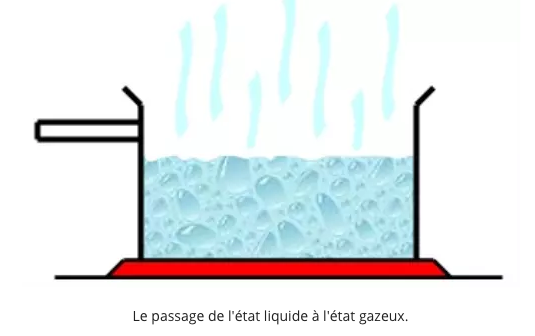
\includegraphics[width=3.491cm,height=2.191cm]{Pictures/10000001000002170000015016F56C8D283134A7.png}La
  liquéfaction : C'est le passage de l'état gazeux à l'état liquide. Ce
  changement d'état s'obtient en cédant de la chaleur. La vapeur devant
  liquide en \emph{cédant de la chaleur.}
\item
  La vaporisation~: de l'eau qui bout dans une casserole ne verra pas sa
  température augmenter avant que toute la quantité d'eau ne soit
  vaporisée. Il faut \emph{apporter de la chaleur} pour que l'eau change
  d'état.
\end{itemize}

\begin{figure}
\centering
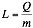
\includegraphics[width=1.177cm,height=0.989cm]{Pictures/10000001000000210000001C2230AC93944A1880.png}
\caption{}
\end{figure}

Exemple~: La chaleur latente\textbf{ de vaporisation} est la quantité de
chaleur qu'il faut \emph{fournir} à 1~kg de liquide (à pression et
température constantes) pour obtenir 1~kg de vapeur.

\emph{\textbf{EXERCICE RESOLU A REALISER page 167. }}

\emph{\textbf{En résumé }}

Le graphique ci-dessous représente la variation de température d'un
corps en fonction du temps.

\begin{figure}
\centering
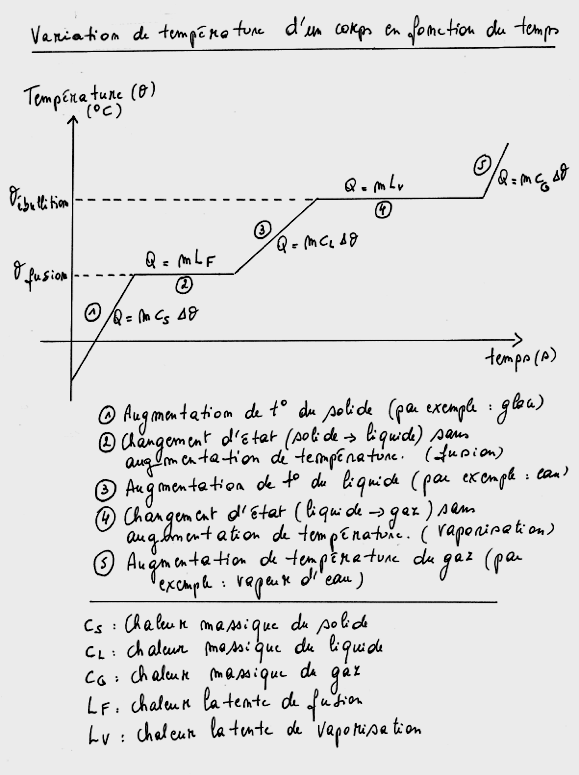
\includegraphics[width=11.084cm,height=11.345cm]{Pictures/100000010000024300000307D0F0277ED39C03FA.png}
\caption{}
\end{figure}

\emph{\textbf{Exemple: Calculer la quantité de chaleur pour transformer
10 g de glace à - 40 °C en 10 g de vapeur d'eau à 120 °C.}}\\
La quantité de chaleur nécessaire pour transformer une masse d'eau
solide à une température \textsubscript{1} en une masse d'eau gazeuse à
une température \textsubscript{2} résulte des cinq transformations
suivantes:\\
• Chauffage de la glace de - 40~ à 0 °C:
\textbf{Q}\textsubscript{\textbf{1}}\textbf{ =
M.C}\textsubscript{\textbf{s}}\textbf{.(0-(-40)) =
M.C}\textsubscript{\textbf{s}}\textbf{.40}\\
• Transformation de la glace en eau liquide à 0 °C:
\textbf{Q}\textsubscript{\textbf{2}}\textbf{ =
M.L}\textsubscript{\textbf{F}}\\
• Chauffage de l'eau liquide de 0~ à 100 °C: Q\textsubscript{3} =
\textbf{M.C}\textsubscript{\textbf{L}}\textbf{.(100-0)=M.C}\textsubscript{\textbf{L}}\textbf{.100}\\
• Transformation de l'eau liquide en vapeur d'eau à 100 °C:
\textbf{Q}\textsubscript{\textbf{4}}\textbf{ =
M.L}\textsubscript{\textbf{V}}\\
• Chauffage de la vapeur d'eau de~ 100 à 120 °C: Q\textsubscript{5} =
\textbf{M.C}\textsubscript{\textbf{G}}\textbf{.(120-100)=M.C}\textsubscript{\textbf{G}}\textbf{.20}\\
~\\
La quantité de chaleur totale est:

Q =~ Q\textsubscript{1} + Q\textsubscript{2}~ +~ Q\textsubscript{3 }+~~~
Q\textsubscript{4}~ +~ Q\textsubscript{5}

Q = M.C\textsubscript{S}(\textsubscript{F} - \textsubscript{1}) +
M.L\textsubscript{F} + M.C\textsubscript{L}(\textsubscript{E} -
\textsubscript{F}) + M.L\textsubscript{V} +
M.C\textsubscript{G}(\textsubscript{2} -  \textsubscript{E})

Q = 0,010. (2,09.10\textsuperscript{3}.40 + 334.10\textsuperscript{3} +
4,18.10\textsuperscript{3}.100 + 2~255.10\textsuperscript{3} +
1,88.10\textsuperscript{3}.20) = \textbf{31 282 J}\\
~\\
Ce calcul peut se généraliser à n'importe quelle substance en faisant
agir les températures de changement d'état.

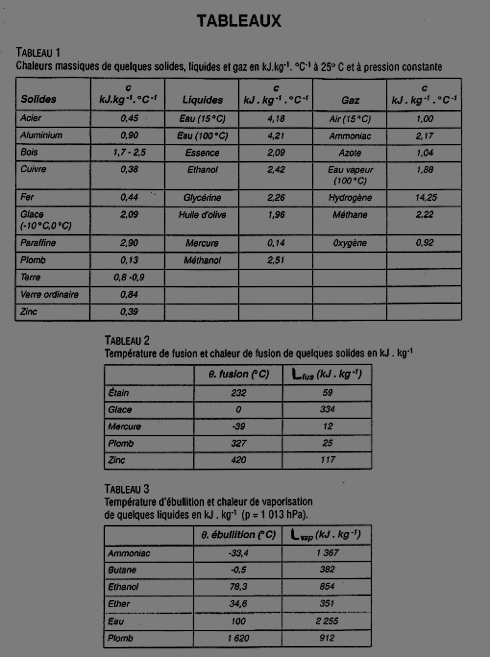
\includegraphics[width=17.851cm,height=23.895cm]{Pictures/10000001000001EA000002916122DCB2747A02B4.png}ANNEXE~:
Chaleurs massiques et latentes de quelques matériaux.

Voir exercice (résolus) en fin de dossier.

\emph{\textbf{B~-- Transformation d'énergie thermique et machines
thermiques}}

Les machines thermiques~sont des machines qui transforment l'énergie
thermique en énergie mécanique \textbf{(moteur à essence, centrale
électrique thermique, machine frigorifique, pompe à chaleur,
turboréacteurs des avions). }

Les premières machines thermiques furent les machines à vapeur ( James
Watt -- 1770) qui contribuèrent à la révolution industrielle . Vinrent
ensuite le moteur à essence (Otto -- 1876) et le moteur diesel (Diesel -
1893).

\emph{\textbf{B.1 -- MACHINES THERMIQUES}}

\emph{\textbf{a) Fonctionnement simplifié d'une machine thermique. }}

\begin{figure}
\centering
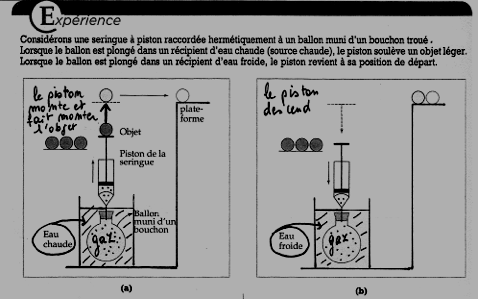
\includegraphics[width=16.558cm,height=10.349cm]{Pictures/10000001000001DE0000012B86B99364138CE2C8.png}
\caption{}
\end{figure}

Le ballon rempli de gaz relié hermétiquement à la seringue est appelé
\textbf{le système.}

Ce dispositif servait à remonter le charbon dans les mines.

\emph{1}\textsuperscript{\emph{er}}\emph{ temps~(fig.a):}

\begin{itemize}
\tightlist
\item
  Une source chaude chauffe le système. (source chaude~: Q1)
\item
  Le gaz se dilate et l'augmentation de pression fait monter le piston.
  Il y a donc transformation d'énergie thermique en travail (W).
\end{itemize}

\emph{2}\textsuperscript{\emph{è}}\emph{ temps(fig.b)~: }

\begin{itemize}
\tightlist
\item
  Le système est refroidi (source froide~: Q2). En effet, pour que la
  machine puisse monter d'autres objets, il faut faire redescendre le
  piston. Le système doit revenir à son état initial.
\end{itemize}

Le cycle de montée--descente peut recommencer. Nous avons donc un
mouvement de va-et-vient~: un cycle.

Pour qu'une machine thermique puisse fonctionner, il faut disposer de
deux sources~: une source chaude et une source froide.

Bilan des échanges d'énergie~: Q1 = W + Q2

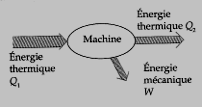
\includegraphics[width=8.348cm,height=4.422cm]{Pictures/10000001000000CA0000006B3AF24511F34B3207.png}\emph{\textbf{b)
Bilan des échanges d'énergie. }}

\begin{itemize}
\tightlist
\item
  Q1~: énergie thermique que le système reçoit (source chaude).
\item
  W~: travail effectué par le système.
\item
  Q2~: énergie thermique perdue par le système (source froide).
\end{itemize}

Si nous admettons qu'à la fin de son cycle, le système est revenu à son
état initial~:

\textbf{L'énergie thermique reçue par le système est égale à l'énergie
cédée sous forme d'énergie mécanique et thermique~: }

\textbf{Q1 = W + Q2  W = Q1 -- Q2}

\emph{\textbf{c) Rendement d'une machine thermique }}

\emph{\textbf{Il apparaît donc qu'une machine thermique ne peut
convertir la totalité de l'énergie thermique Q1 qui lui est fournie en
énergie mécanique W. Il y a nécessairement une partie de l'énergie
thermique qui part vers la source froide (sans quoi, il n'y a pas de
cycle). }}

Or, c'est bien l'énergie mécanique qui est recherchée par l'utilisateur.

\emph{Rendement  d'une machine thermique~: }

\emph{Remarques~: }

\begin{itemize}
\tightlist
\item
  Si T2 est proche de T1, le rendement tend vers 0. Pour augmenter le
  rendement d'une machine thermique, il faut une grande différence de
  température entre la source chaude et la source froide.
\item
  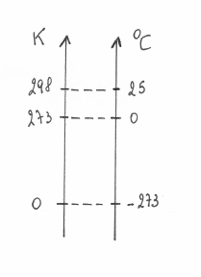
\includegraphics[width=3.293cm,height=4.538cm]{Pictures/10000001000000C90000011558FC2D6C1A163765.png}Si
  T1  T2, le rapport T2/T1 tend vers zéro et le rendement vers 100\%.
  Pour augmenter le rendement d'une machine thermique, il faut une
  grande différence de température entre la source chaude et la source
  froide.
\end{itemize}

\emph{Rappel}~: conversion de degré Celsius en degré Kelvin~:

\emph{\textbf{B.2 -- MOTEURS}}

\begin{enumerate}
\def\labelenumi{\alph{enumi})}
\tightlist
\item
  \emph{\textbf{Le moteur à essence (pages 170-171). }}
\end{enumerate}

Le moteur à essence est une machine thermique puisqu'il transforme une
énergie thermique en énergie mécanique.

La source chaude résulte de la combustion du mélange air - essence.

La source froide est l'atmosphère. Le rendement d'un moteur est donc
plus performant par temps froid.

Dans la grande majorité des cas, un moteur possède 4 cylindres.

Chaque cylindre est relié au vilebrequin
(\href{https://fr.wikipedia.org/wiki/Cat\%C3\%A9gorie:Dispositif_m\%C3\%A9canique}{\emph{\emph{dispositif
mécanique}}} qui permet la transformation du mouvement linéaire
rectiligne du piston en un
\href{https://fr.wikipedia.org/wiki/Mouvement_de_rotation}{\emph{\emph{mouvement
de rotation}}} continu.

Le moteur thermique d'une voiture fonctionne en quatre étapes. On dit
donc qu'il s'agit d'un moteur à quatre temps.

Dans le moteur sont creusés des cylindres et à l'intérieur de chaque
cylindre se trouve un piston.

\begin{enumerate}
\def\labelenumi{\arabic{enumi}.}
\tightlist
\item
  \textbf{Admission~}: les pistons descendent, aspirant du carburant et
  de l'air.
\item
  \textbf{Compression - explosion~}: en remontant, tout ce mélange est
  comprimé dans les cylindres.
\item
  \textbf{Détente}~: arrivé en haut, il se produit une combustion de ce
  mélange grâce à une étincelle. Cette explosion renvoie alors les
  pistons vers le bas.
\item
  \textbf{Echappement}~: les pistons remonteront à nouveau pour pousser
  les gaz d'échappement vers l'extérieur du moteur. Le cycle
  recommencera alors de zéro.
\end{enumerate}

Ce mouvement de va et vient fait tourner un axe qui sort du moteur pour
aller jusqu'aux roues. Voici donc comment le moteur thermique d'une
voiture permet son fonctionnement.

\begin{figure}
\centering
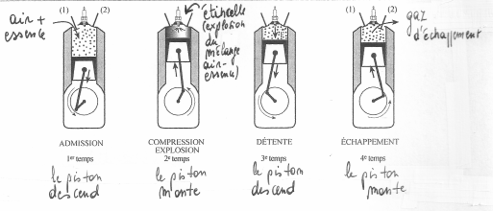
\includegraphics[width=15.946cm,height=6.844cm]{Pictures/10000001000001ED000000D356E01F68F1130F39.png}
\caption{}
\end{figure}

\begin{enumerate}
\def\labelenumi{\alph{enumi})}
\tightlist
\item
  \emph{\textbf{La centrale thermique classique}}
\end{enumerate}

\begin{enumerate}
\def\labelenumi{\arabic{enumi})}
\tightlist
\item
  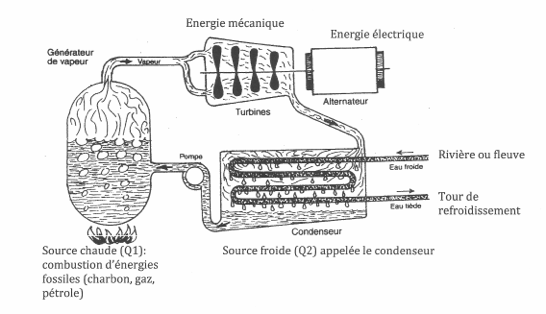
\includegraphics[width=17.851cm,height=10.278cm]{Pictures/10000001000002220000013A629B591569517346.png}\textbf{Une
  combustion a lieu dans la chaudière} et chauffe de l'eau qui se
  transforme en vapeur.
\end{enumerate}

Ces centrales brûlent des énergies fossiles (charbon, fioul, gaz et donc
émission de CO\textsubscript{2} dans l'atmosphère) ( transformation
d'énergie chimique en énergie thermique).

\begin{enumerate}
\def\labelenumi{\arabic{enumi})}
\tightlist
\item
  \textbf{La vapeur surchauffée fait tourner une turbine} (conversion
  d'énergie thermique en énergie mécanique). Cette turbine actionnera un
  alternateur pour transformer l'énergie mécanique en énergie
  électrique.
\item
  \textbf{La vapeur est ensuite refroidie par de l'eau froide} dans le
  condenseur.
\item
  \textbf{L'eau de condensation est renvoyée dans la chaudière. }L'eau
  froide qui a servi à la condensation ressort tiède, (elle emporte Q2).
  Afin de ne pas rejeter une eau tiède dans l'environnement, elle est
  refroidie dans de gigantesques tours de refroidissement.
\end{enumerate}

\emph{Rappel~: Fonctionnement de l'alternateur. }

Un aimant est mobile à proximité d'une bobine de fil de cuivre induit un
courant électrique dans la bobine et on peut l'utiliser pour alimenter
un circuit électrique.

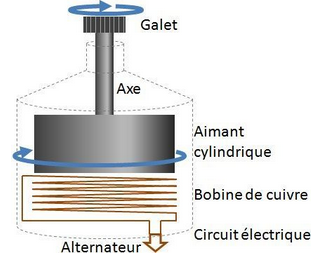
\includegraphics[width=6.424cm,height=5.339cm]{Pictures/10000001000001380000010305BEE511D6A017FC.png}Dans
le cas d'une centrale thermique, c'est le mouvement de rotation de l'axe
de la turbine qui génère le mouvement de l'aimant dans la bobine de
l'alternateur.

Il y a production d'énergie électrique qui est envoyée sur le réseau.

\begin{enumerate}
\def\labelenumi{\alph{enumi})}
\tightlist
\item
  \emph{\textbf{Machines frigorifiques et pompe à chaleur.}}
\end{enumerate}

Les machines frigorifiques refroidissent l'intérieur d'une enceinte en
réchauffant le milieu dans lequel elles se trouvent et les pompes à
chaleur font l'inverse.

Elles utilisent un fluide frigorigène (ou réfrigérant). C'est un
\href{https://fr.wikipedia.org/wiki/Fluide_(mati\%C3\%A8re)}{\emph{\emph{fluide}}}
qui permet la mise en œuvre d'un
\href{https://fr.wikipedia.org/wiki/Cycle_frigorifique}{\emph{\emph{cycle
thermique}}}. Ce fluide absorbe la chaleur à basse température et basse
pression, puis libère la chaleur à une température et une pression plus
élevées, généralement par un changement d'état. Les fluides frigorigènes
sont utilisés dans les systèmes de
\href{https://fr.wikipedia.org/wiki/R\%C3\%A9frig\%C3\%A9ration}{\emph{\emph{production
de froid}}} (climatisation, congélateur, réfrigérateur,~etc.), comme
dans les systèmes de production de chaud par
\href{https://fr.wikipedia.org/wiki/Pompe_\%C3\%A0_chaleur}{\emph{\emph{pompes
à chaleur}}}.

\emph{Rappel~: }

\begin{itemize}
\tightlist
\item
  La \textbf{vaporisation(ou évaporation)}, qui est le changement d'état
  d'un fluide \textbf{de l'état liquide à l'état gazeux}, est un
  phénomène \textbf{endothermique}. Le fluide prend de la chaleur à son
  environnement pour réaliser ce changement d'état. (Il faut chauffer de
  l'eau pour la vaporiser).
\end{itemize}

\begin{itemize}
\tightlist
\item
  La \textbf{liquéfaction},~qui est le changement d'état d'un fluide de
  \textbf{l'état gazeux à l'état liquide}, est un phénomène
  \textbf{exothermique}. Le fluide cède de la chaleur dans son
  environnement en réalisant ce changement d'état. (Il faut refroidir de
  la vapeur d'eau pour la liquéfier).
\end{itemize}

\emph{\textbf{Ces deux changements d'état, l'un exothermique, l'autre
exothermique, sont la base du principe de fonctionnement des machines
frigorifiques et pompes à chaleur. }}

\textbf{}

\textbf{}

\textbf{}

\textbf{}

\textbf{}

\textbf{}

\textbf{}

\textbf{}

\textbf{}

\textbf{}

\textbf{}

\textbf{}

\textbf{\emph{\textbf{c.1) Le réfrigérateur }}}

\textbf{}

\textbf{\emph{\textbf{Principe de fonctionnement du réfrigérateur}}}

\textbf{\textbf{Principe de base~: on refroidit l'intérieur de
l'appareil et on réchauffe la pièce où se trouve le réfrigérateur. }}

\textbf{\textbf{Pour réaliser ces transferts de chaleur, on utilise un
intermédiaire, un fluide que l'on fait passer alternativement de l'état
gazeux à l'état liquide et inversement. On s'arrange pour que ce fluide
réalise un circuit et s'évapore (et donc refroidisse l'environnement) à
l'intérieur du réfrigérateur tout en se liquéfiant à l'extérieur (et
donc échauffe l'environnement). }}

\textbf{}

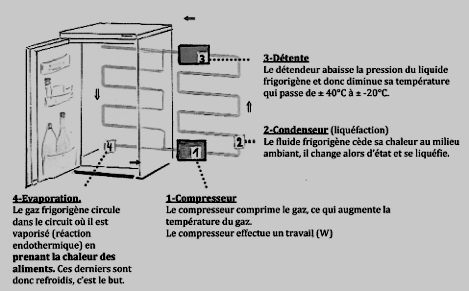
\includegraphics[width=14.263cm,height=8.848cm]{Pictures/10000001000001D50000012367CA7DC2A31818DF.png}\textbf{}

\textbf{\textbf{}}

\textbf{}

\textbf{}

\textbf{}

\textbf{}

\textbf{}

\textbf{}

\textbf{}

\textbf{}

\textbf{}

\textbf{\textbf{}}

\textbf{}

\textbf{}

\textbf{}

\textbf{}

\textbf{}

\textbf{}

\textbf{}

\textbf{}

\textbf{}

\textbf{\emph{\textbf{1 -- Compresseur.}}}

\begin{quote}
\textbf{\textbf{Pour faire circuler le fluide de l'intérieur vers
l'extérieur du réfrigérateur, on utilise un compresseur qui aspire
d'abord le gaz, le comprime et le refoule à l'extérieur. Le gaz se
transforme en vapeur à haute pression et haute température. }}
\end{quote}

\begin{quote}
\textbf{\textbf{Le compresseur fonctionne comme une pompe et fournit un
travail (W).}}
\end{quote}

\textbf{\textbf{}\emph{\textbf{2- Condenseur.}}}

\begin{quote}
\textbf{\textbf{Cette vapeur et dirigée vers le condenseur (un long
serpentin en contact avec l'air ambiant plus froid (à l'extérieur du
réfrigérateur). La vapeur va donc se condenser sur les parois du
serpentin tout en cédant de la chaleur à l'air extérieur. A la sortie du
condenseur, le fluide est devenu liquide et s'est un peu refroidi. .
C'est le premier changement d'état.}}
\end{quote}

\textbf{\textbf{}\emph{\textbf{3 -- Détendeur.}}}

\begin{quote}
\textbf{\textbf{Le fluide passe ensuite dans le détendeur~: dispositif
qui diminue brutalement la pression du fluide avec pour conséquence une
baisse importante de la température en dessous de celle que l'on veut
maintenir à l'intérieur du réfrigérateur. }}
\end{quote}

\begin{quote}
\textbf{\textbf{Rappel~: diminuer la pression d'un gaz diminue sa
température.}}
\end{quote}

\textbf{\emph{\textbf{4 - Evaporation.}}}

\begin{quote}
\textbf{\textbf{Ce liquide entre dans le réfrigérateur et arrive dans
l'évaporateur qui, comme le condenseur, est un long serpentin qui met le
fluide en contact avec l'air à l'intérieur du frigo. Cet air est plus
chaud que le fluide et donc ce fluide recevant de la chaleur (les
aliments dans le frigo sont plus chauds que le fluide), va se
transformer en gaz (il se vaporise) en extrayant la chaleur de l'air
ambiant (provenant de la chaleur des aliments). L'intérieur du
réfrigérateur se refroidit.}}
\end{quote}

\textbf{}

\textbf{\textbf{Et le cycle recommence. }}

\textbf{}

\emph{\textbf{Bilan énergétique du réfrigérateur et rendement}}

\begin{figure}
\centering
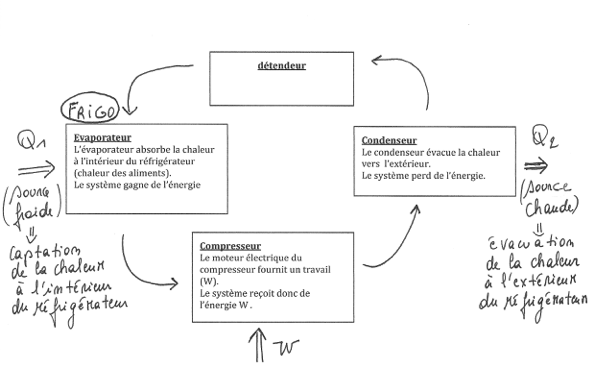
\includegraphics[width=12.771cm,height=7.902cm]{Pictures/100000010000025300000171E55891644F01868A.png}
\caption{}
\end{figure}

En vertu du principe de conservation\textbf{ }d'énergie,\textbf{ }le
système étant le fluide qui circule, les énergies reçues par le système
sont égales à l'énergie cédée.

L'énergie utile est Q1 et l'énergie investie W. On peut donc exprimer
\emph{\textbf{le rendement}} sous la forme~:

\emph{\textbf{c.2. La pompe à chaleur}}

La pompe à chaleur est utilisée comme procédé d'énergie de chauffage.

La pompe à chaleur fonctionne de la même façon qu'un réfrigérateur.

Un fluide très volatil circule dans un circuit fermé. Dans ce cas, le
condenseur est dans la maison et l'évaporateur à l'extérieur.

La partie à l'extérieur est en contact avec le sol, de l'eau ou de
l'air.

\begin{figure}
\centering
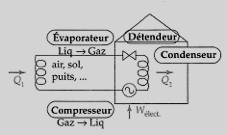
\includegraphics[width=6.008cm,height=3.739cm]{Pictures/10000001000000E30000008754ECBE984DD7350E.png}
\caption{}
\end{figure}

\emph{\textbf{Bilan énergétique de la pompe à chaleur et rendement}}

En vertu du principe de conservation\textbf{ }d'énergie,\textbf{ }le
système étant le fluide qui circule, les énergies reçues par le système
sont égale à l'énergie cédée (comme pour le réfrigérateur).

Puisque l'énergie thermique extérieure (Q1) est illimitée et que l'on
paie moins d'énergie (W) que l'on en reçoit (Q2), le rendement est
supérieur à 1. Il est généralement appelé «~COP~», coefficient de
performance.

Une pompe à chaleur de COP égal à 4 utilise 1 kwh électrique (W) pour 4
kwh thermique (Q2). Ce qui signifie que trois quarts de l'énergie de
chauffage (Q1) provient d'une source gratuite et renouvelable.

NB~: 1 kwh = 1000w.3600s = 3,6.10\textsuperscript{6} ws =
3,6.10\textsuperscript{6} J

Le COP est d'autant plus grand que la température extérieure est faible.
C'est pourquoi on utilise de préférence le sol extérieur en
hiver~(température constante de 8°C à 1 mètre de profondeur).

La pompe à chaleur est donc très intéressante d'un point de vue
énergétique. Son inconvénient est le coût relativement élevé de
l'installation par rapport au chauffage classique par combustion
d'énergies fossiles (chaudières).

\begin{figure}
\centering
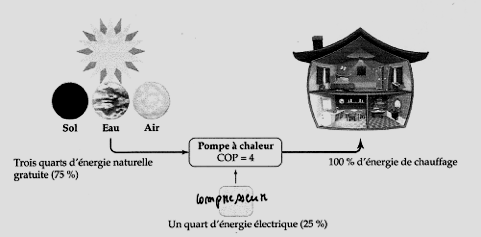
\includegraphics[width=17.898cm,height=8.819cm]{Pictures/10000001000001E1000000ED8743610641ABBB0F.png}
\caption{}
\end{figure}

\emph{\textbf{Exercices de calorimétrie}}

\emph{\textbf{Exercice 1}}

Quelle est la quantité d'énergie calorifique nécessaire pour faire
fondre 300 g de glace, sachant que la chaleur latente de la glace est de
334~ kJ/kg.°C? (rép. 100,2 kJ)

\emph{\textbf{Exercice 2}}

Quelle quantité de chaleur faut-il fournir à une masse de 1 kg d'huile
pour élever sa température de 10° C~sachant que la chaleur massique de
l'huile est de 1960 J/kg.°C?

(rép. 19,6 kJ)

\emph{\textbf{Exercice 3}}

Quelle quantité de chaleur faut-il fournir à une masse de 1 kg d'eau
liquide pour élever sa température de 10° C~sachant que la chaleur
massique de l'eau liquide est de 4186 J/kg.°C?

(rép.41,9 kJ)

\emph{\textbf{Exercice 4}}

On fournit 20 kJ à 200 g d'eau liquide qui a une température de 20°C.
Quelle sera la température finale~? (rép. 43,9°C)

\emph{\textbf{Exercice 5}}

Quelle est la quantité d'énergie calorifique nécessaire pour vaporiser
600 g d'éthanol~sachant que la chaleur latente de l'éthanol est de 850
kJ/kg~? (rép. 510 kJ)

\emph{\textbf{Exercice 6}}

Quelle est la quantité d'énergie calorifique nécessaire pour transformer
complètement 500 g de glace à -10°C en vapeur à 100°C~? (rép. 1514,25
kJ).

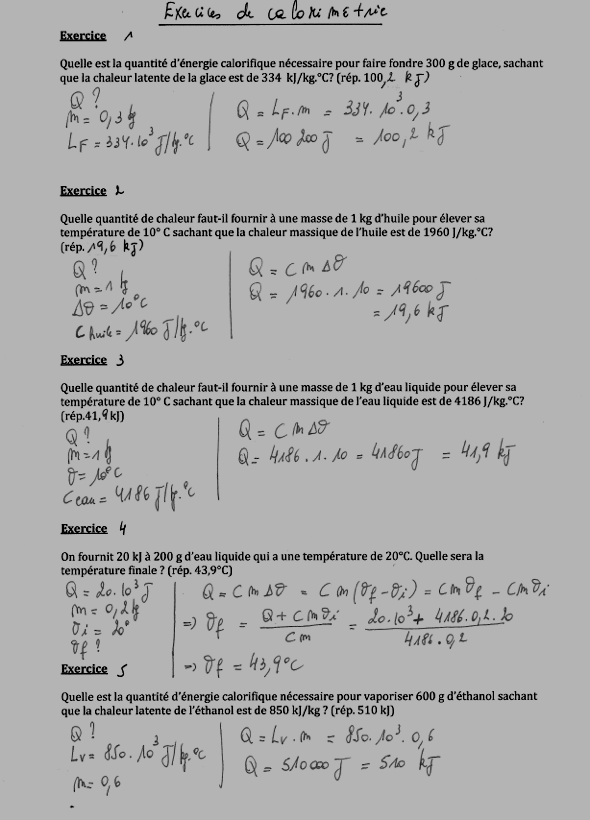
\includegraphics[width=18.486cm,height=25.73cm]{Pictures/100000010000024E00000334339B3944B6446F24.png}

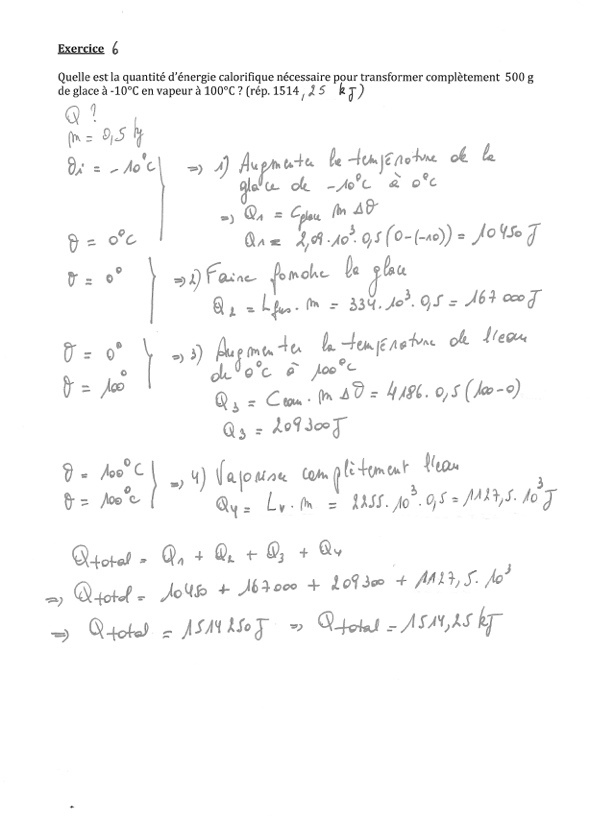
\includegraphics[width=18.486cm,height=25.73cm]{Pictures/100000010000024E000003341A59B4106578A675.png}

\emph{\textbf{Machines thermiques -- Exercices}}

\emph{\textbf{Exercice 1}}

Une machine thermique simple fonctionne avec deux sources de chaleur,
une source chaude (Q1) et une source froide (Q2).

Si les températures respectives sont~: t1=70°C et t2=15°C, calculer le
rendement théorique de cette machine.

\emph{\textbf{Exercice 2 (N°3 page 184)}}

Evaluer approximativement l'élévation de température d'une balle de
fusil qui pénètre et s'arrête dans un paquet de sable si~:

\begin{itemize}
\tightlist
\item
  la vitesse initiale de la balle est de 600 m/s,
\item
  la masse de la balle est de 20 g,
\item
  la chaleur massique du métal (fer, acier) est de 450 J/kg.°C,
\item
  la température initiale est proche de 15°C.
\end{itemize}

\emph{\textbf{Exercice 3}}

Un réchaud électrique possède une puissance de 1000 W. Il sert à
chauffer un volume V=1L d'eau de 14°C à l'ébullition. Sachant que 60\%
de la chaleur dégagée par le réchaud est emmagasinée par l'eau, calculer
la durée du chauffage.

\emph{\textbf{Exercice 4}}

Combien de temps fait-il à un réchaud d'une puissance de 500 W pour
faire passer 400 g d'eau de 15°C à 98°C~?

\emph{\textbf{Exercice 5}}

Un camion de 25 tonnes roule à 90 km/h, lorsqu'il doit freiner
brusquement jusqu'à l'arrêt. On suppose que 80\% de l'énergie cinétique
est convertie en énergie thermique des freins.

Quelle doit être la masse des disques de freins en fer
(c\textsubscript{fer}=450 J/kg.°C) si l'échauffement ne doit pas
dépasser =400C~?

\emph{\textbf{Exercice 6 (N°7 page 184)}}

Pendant le week-end du premier mai, un voisin a remis en route le
chauffage de sa piscine en utilisant sa nouvelle pompe à chaleur
récupérant ainsi l'énergie de l'air extérieur à 25°C.

Comparer le gain énergétique de son installation par rapport à un autre
moyen de chauffage de la piscine, par exemple un système de résistance
chauffantes, si~:

-Le rendement de l'installation électrique est de 95\%.

-Le coefficient de performance de la pompe à chaleur est de 4.

-Le volume d'eau à chauffer est de 72m\textsuperscript{3}.

-La température espérée pour l'eau de la piscine est de 30°.

\emph{\textbf{Exercice 7}}

\textbf{Chauffage de l'eau du bassin d'une piscine avec une pompe à
chaleur.}

Après remplissage d'une piscine d'un volume de 560 m\textsuperscript{3}
avec une eau initialement prise à l'extérieur à une température de 17°C,
on souhaite augmenter la température de l'eau jusqu'à 28°C. On
considérera que le transfert thermique depuis la pompe à chaleur sert
intégralement à chauffer l'eau sans déperdition.

\begin{enumerate}
\def\labelenumi{\arabic{enumi})}
\tightlist
\item
  Calculer la valeur Q2, énergie transférée par le fluide de la pompe à
  chaleur à l'eau de la piscine quand la température a atteint 28°C.
\end{enumerate}

\begin{enumerate}
\def\labelenumi{\arabic{enumi})}
\tightlist
\item
  On a mesuré l'énergie thermique We consommée pendant ce transfert et
  trouvé une valeur égale à~: We=8.10\textsuperscript{9} J. déterminer
  la valeur de Q1, l'énergie transférée par l'air extérieur.
\end{enumerate}

\begin{enumerate}
\def\labelenumi{\arabic{enumi})}
\tightlist
\item
  Exprimer, puis calculer le coefficient de performance de la pompe à
  chaleur.
\end{enumerate}

\begin{enumerate}
\def\labelenumi{\arabic{enumi})}
\tightlist
\item
  Montrer qu'avec une pompe à chaleur de coefficient de performance égal
  à 3, on réalise 67\% d'économie sur la facture en énergie électrique
  par rapport à un chauffage direct utilisant, par exemple, une
  résistance électrique.
\end{enumerate}

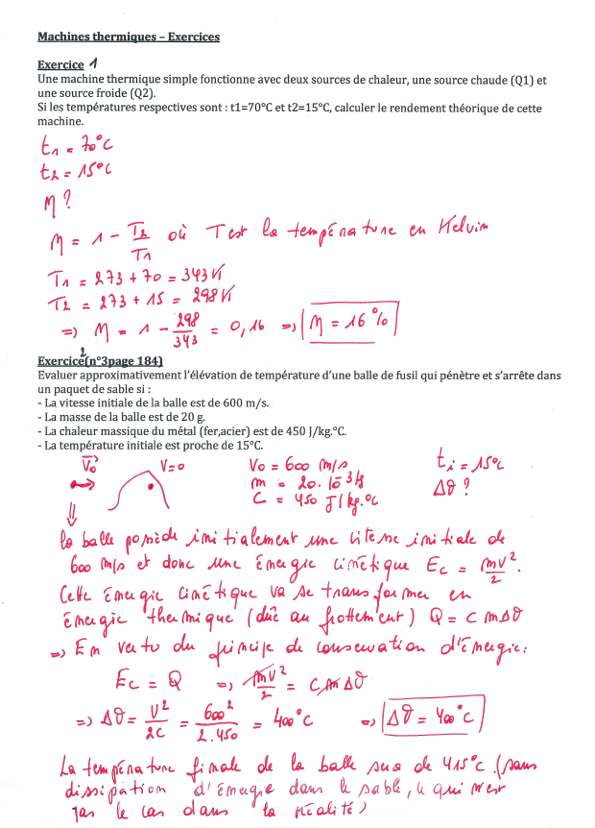
\includegraphics[width=19.239cm,height=26.741cm]{Pictures/10000001000002530000033C4DAAA30BE8CDB504.png}

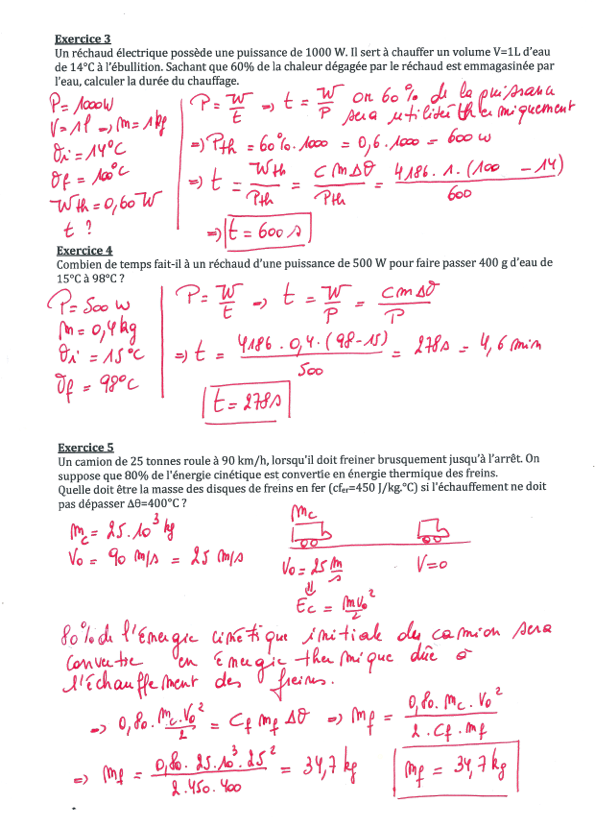
\includegraphics[width=19.239cm,height=26.741cm]{Pictures/10000001000002530000033C5B177CADC8B81C22.png}

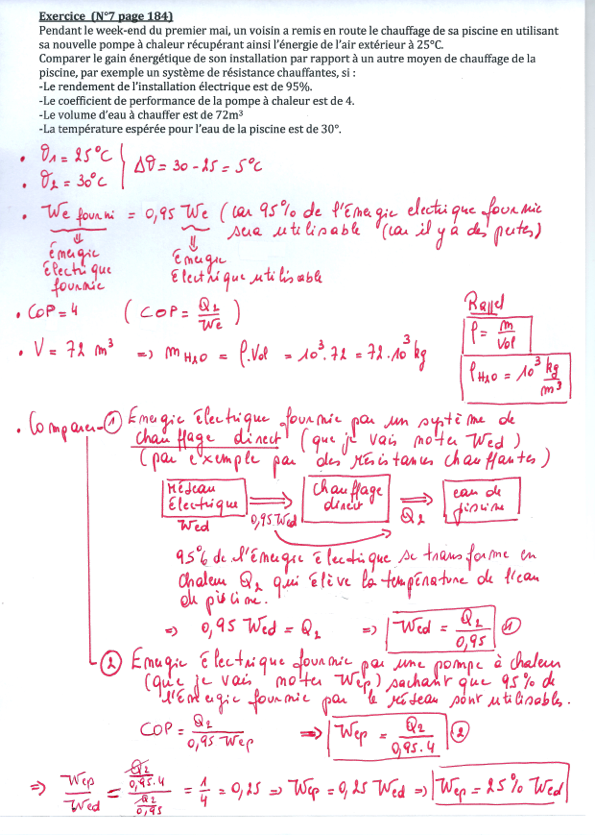
\includegraphics[width=19.239cm,height=26.975cm]{Pictures/100000010000025300000343E75324A8017B0310.png}

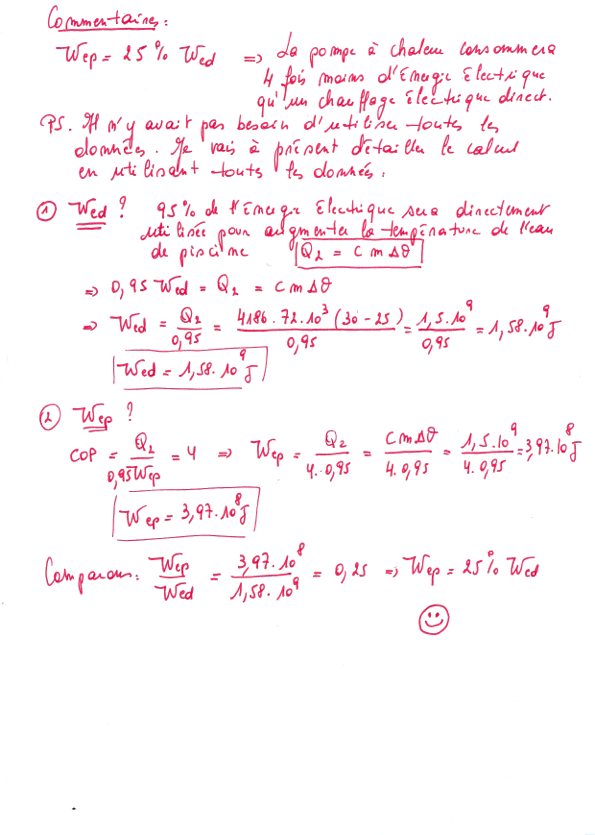
\includegraphics[width=19.239cm,height=26.975cm]{Pictures/100000010000025300000343E2BD3741EC0DE6A2.png}

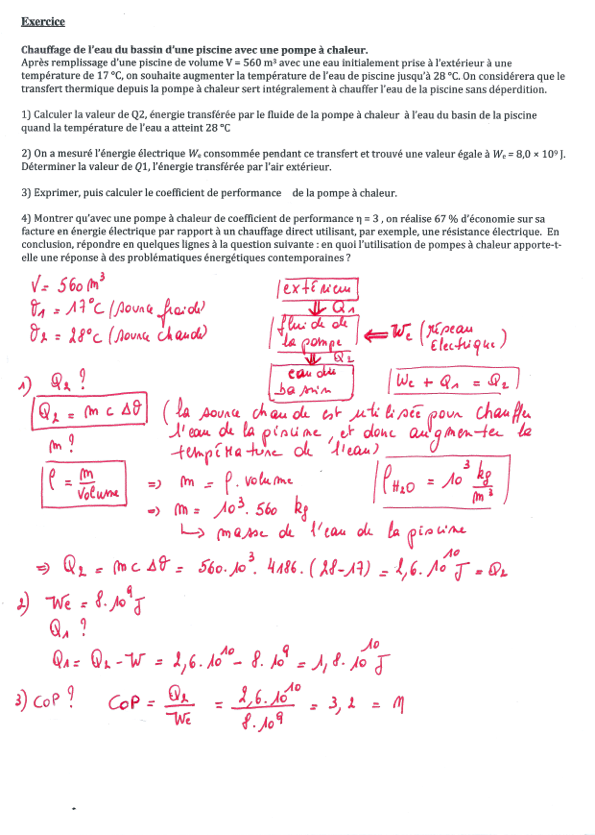
\includegraphics[width=19.239cm,height=26.975cm]{Pictures/100000010000025300000343FDF0776EAA696B9B.png}

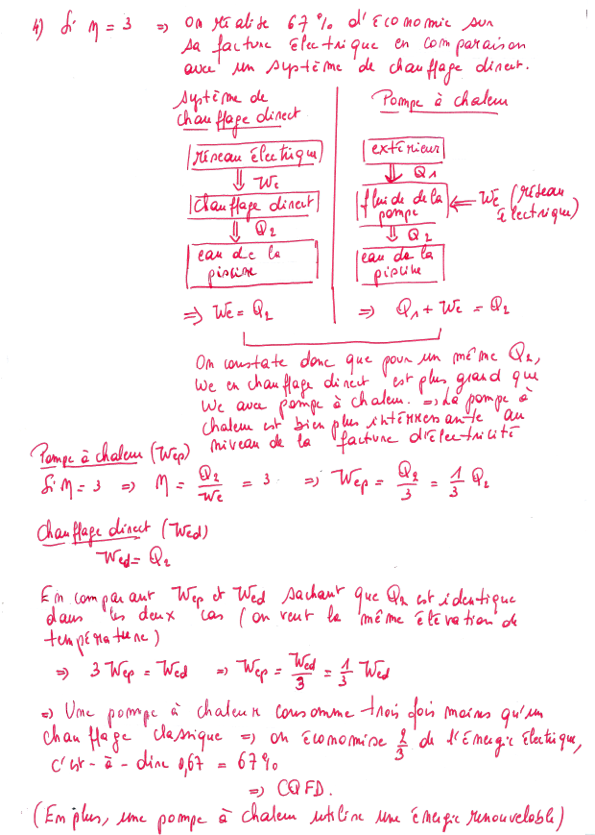
\includegraphics[width=18.251cm,height=25.591cm]{Pictures/1000000100000253000003439D3D805CCD33A9FD.png}

\emph{\textbf{SYNTHESE DE THERMODYNAMIQUE}}

\begin{figure}
\centering
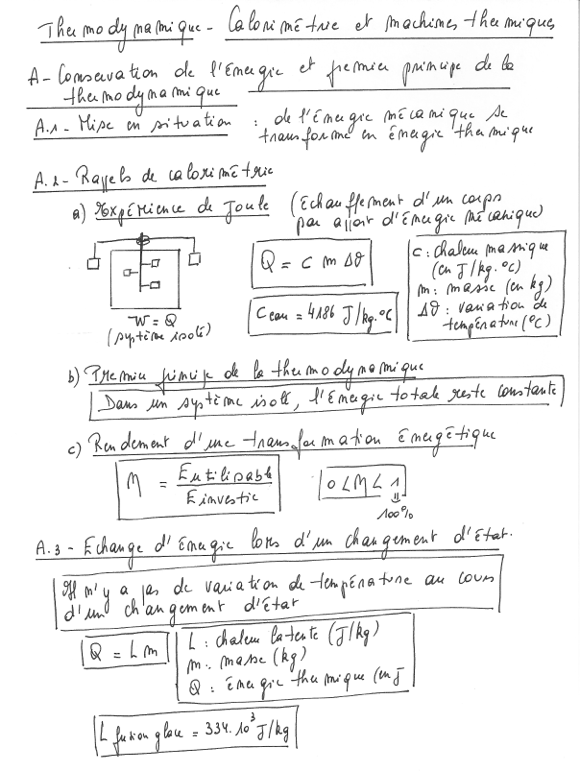
\includegraphics[width=18.486cm,height=24.576cm]{Pictures/1000000100000244000003044E80AD546388D528.png}
\caption{}
\end{figure}

\begin{figure}
\centering
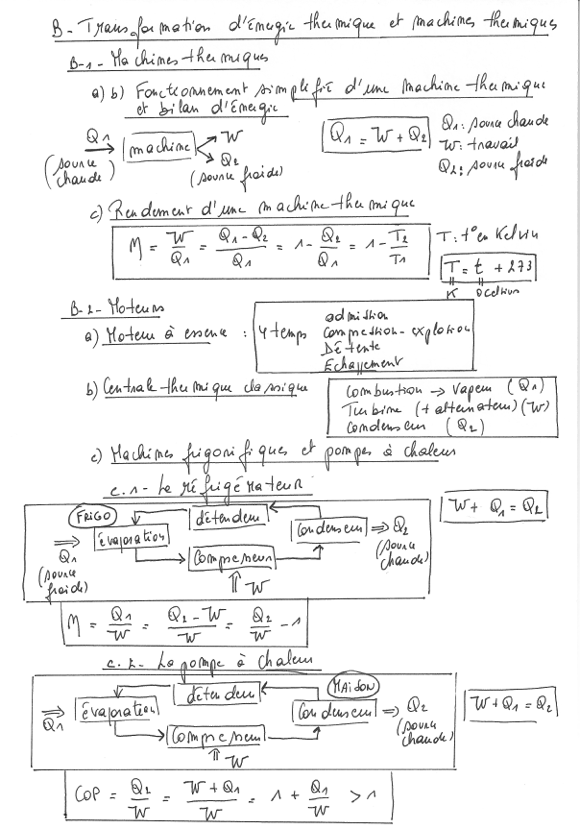
\includegraphics[width=19.143cm,height=27.376cm]{Pictures/10000001000002440000033EFBA46FA2D90A9FB6.png}
\caption{}
\end{figure}
